\section*{Proposed Techniques}

\begin{frame}{Proposed technique: \CPDSearch{}}
    \begin{block}{Idea}
        \A{} variant yielding bounded suboptimal solutions where \CPDPath{} is exploited for online searching the perturbated map.
    \end{block}

    $s$, $t$ : start and target of path finding instance;
    
    $n$: a search node expanded during \CPDSearch{};

    \begin{block}{}
        \begin{itemize}
            \item[-] $\CPDPath{}[n \rightarrow t]$: path from $n$ to $t$ generated from \CPD{} computed with \textbf{original} weights;
            \item[-] $\CPDPathNew{}[n \rightarrow t]$: path from $n$ to $t$ generated from \CPD{} computed with \textbf{perturbated} weights;
        \end{itemize} 
    \end{block}

    cost of a path identified by $cost(\cdot)$;
\end{frame}

\begin{frame}{Proposed technique: \CPDSearch{}}
    \begin{block}{Idea}
        \A{} variant yielding bounded suboptimal solutions where \CPDPath{} is exploited for online searching the perturbated map.
    \end{block}

    \begin{itemize}
        \item {use \CPD{} to derive an admissible heuristic};
    \end{itemize}

    \begin{minipage}{0.65\textwidth}
        \begin{center}
        Perturbations only increases edge costs 
        
        $\downarrow$ 
        
        $cost(\CPDPath{}[n \rightarrow t])$ is an admissible heuristic;

        \medskip

        $cost(\CPDPath{}[2 \rightarrow 6]) = 6$

        $cost(\CPDPathNew{}[2 \rightarrow 6]) = 9$
        \end{center}
    \end{minipage}\hfill%
    \begin{minipage}{0.35\textwidth}
        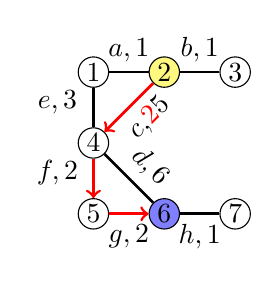
\begin{tikzpicture}
            \tikzset{Vertex/.style={%
                shape=circle,%
                draw=black,%
                minimum size=10pt,%
                radius=0.7cm,%
                inner sep=1pt,%
                node distance=0.9cm,%
            }}
        
            \node[Vertex] (1) {$1$};
            \node[Vertex, right of=1, fill=yellow!50] (2) {$2$};
            \node[Vertex, right of=2] (3) {$3$};
            \node[Vertex, below of=1] (4) {$4$};
            \node[Vertex, below of=4] (5) {$5$};
            \node[Vertex, right of=5, fill=blue!50] (6) {$6$};
            \node[Vertex, right of=6] (7) {$7$};
    
            \path (2) edge[-,line width=1pt] node[above]{\color{black}$a,1$} (1);
            \path (2) edge[-,line width=1pt] node[above]{\color{black}$b,1$} (3);
            \path (2) edge[->,line width=1pt, color=red] node[below,sloped,pos=0.4]{{\color{black} $c,$}{\color{red} \xcancel{2}}{\color{black}5}} (4);
            \path (4) edge[-,line width=1pt] node[above,sloped,pos=0.6]{\color{black}$d,6$} (6);
            \path (1) edge[-,line width=1pt] node[above,xshift=-13pt,yshift=-6pt]{\color{black}$e,3$} (4);
            \path (4) edge[->,line width=1pt, color=red] node[above,xshift=-13pt, yshift=-6pt]{\color{black}$f,2$} (5);
            \path (5) edge[->,line width=1pt, color=red] node[below]{\color{black}$g,2$} (6);
            \path (6) edge[-,line width=1pt] node[below]{\color{black}$h,1$} (7);
        \end{tikzpicture}
    \end{minipage}

\end{frame}

\begin{frame}{Proposed technique: \CPDSearch{}}
    \begin{block}{Idea}
        \A{} variant yielding bounded suboptimal solutions where \CPDPath{} is exploited for online searching the perturbated map.
    \end{block}

    \begin{itemize}
        \item {\color{gray}use \CPD{} to derive an admissible heuristic;}
        \item {use \CPD{} for a (early) search termination;}
    \end{itemize}

    \begin{minipage}{0.65\textwidth}

        \begin{center}
            if $cost(\CPDPathNew{}[n \rightarrow t]) = cost(\CPDPath{}[n \rightarrow t])$
            
            $\downarrow$
            
            optimal solution is $path[s \rightarrow n] \doublePlus{} \CPDPath{}[n \rightarrow t]$;

            \medskip

            $(s, t) = (2, 6)$
        
            $cost(\CPDPath{}[4 \rightarrow 6]) = 4$

            $cost(\CPDPathNew{}[4 \rightarrow 6]) = 4$
        \end{center}
    \end{minipage}\hfill%
    \begin{minipage}{0.35\textwidth}
        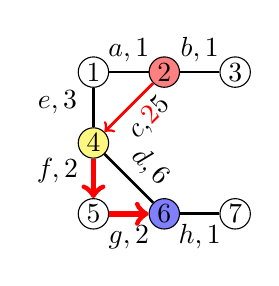
\begin{tikzpicture}
            \tikzset{Vertex/.style={%
                shape=circle,%
                draw=black,%
                minimum size=10pt,%
                radius=0.7cm,%
                inner sep=1pt,%
                node distance=0.9cm,%
            }}
        
            \node[Vertex] (1) {$1$};
            \node[Vertex, right of=1, fill=red!50] (2) {$2$};
            \node[Vertex, right of=2] (3) {$3$};
            \node[Vertex, below of=1, fill=yellow!50] (4) {$4$};
            \node[Vertex, below of=4] (5) {$5$};
            \node[Vertex, right of=5, fill=blue!50] (6) {$6$};
            \node[Vertex, right of=6] (7) {$7$};
    
            \path (2) edge[-,line width=1pt] node[above]{\color{black}$a,1$} (1);
            \path (2) edge[-,line width=1pt] node[above]{\color{black}$b,1$} (3);
            \path (2) edge[->,line width=1pt, color=red] node[below,sloped,pos=0.4]{{\color{black} $c,$}{\color{red} \xcancel{2}}{\color{black}5}} (4);
            \path (4) edge[-,line width=1pt] node[above,sloped,pos=0.6]{\color{black}$d,6$} (6);
            \path (1) edge[-,line width=1pt] node[above,xshift=-13pt,yshift=-6pt]{\color{black}$e,3$} (4);
            \path (4) edge[->,line width=2pt, color=red] node[above,xshift=-13pt, yshift=-6pt]{\color{black}$f,2$} (5);
            \path (5) edge[->,line width=2pt, color=red] node[below]{\color{black}$g,2$} (6);
            \path (6) edge[-,line width=1pt] node[below]{\color{black}$h,1$} (7);
        \end{tikzpicture}
    \end{minipage}

\end{frame}

\begin{frame}{Proposed technique: \CPDSearch{}}
    \begin{block}{Idea}
        \A{} variant yielding bounded suboptimal solutions where \CPDPath{} is exploited for online searching the perturbated map.
    \end{block}

    \begin{itemize}
        \item {\color{gray}use \CPD{} to derive an admissible heuristic;}
        \item {\color{gray}use \CPD{} for a (early) search termination;}
        \item {use \CPD{} to obtain solution bounds;}
    \end{itemize}

    Given source $s$, target $t$ and search node $n$: 
    \begin{itemize}
        \item[-] $cost(path[s \rightarrow n] \doublePlus{} \CPDPath{}[n \rightarrow t])$: lowerbound of solution;
        \item[-] $cost(path[s \rightarrow n] \doublePlus{} \CPDPathNew{}[n \rightarrow t])$: upperbound of solution;
    \end{itemize}

    \begin{block}{}
        \begin{itemize}
            \item \CPDSearch{} maintains the best solution found and solution bounds (allows usage in anytime search);
            \item Threshold $\epsilon$ used for setting \CPDSearch{} solution quality (we focus on $\epsilon = 1 \rightarrow $ optimality);
        \end{itemize}
    \end{block}

\end{frame}

